\documentclass{article}

% Paper setting
\usepackage[utf8]{inputenc}
\usepackage[vietnamese=nohyphenation]{hyphsubst}
\usepackage[english,vietnamese]{babel}

\usepackage[fontsize=13pt]{scrextend}
\usepackage[a4paper, portrait, margin=2.5cm]{geometry}

% \linespread{1.25}
\usepackage{setspace}
\usepackage{times}
\usepackage{afterpage}
\usepackage{listings}

% Table of contents
\usepackage[nottoc]{tocbibind}

% Icons for subitems in lists
\renewcommand{\labelitemii}{$\circ$}

% References
% \usepackage{natbib}
% \bibliographystyle{humannat}
% \setcitestyle{authoryear,open={(},close={)}}
\usepackage[style=authoryear,sorting=nyt,bibencoding=auto,backend=biber,autolang=other]{biblatex}
\bibliography{my_bib.bib}
\renewcommand*{\nameyeardelim}{\addcomma\space}

% Frame for title page
\usepackage[most]{tcolorbox}

% Maths
\usepackage{amsmath}

% Image & figures
\usepackage{graphicx}
\usepackage[labelfont=bf]{caption}
\usepackage{subcaption}

% Cool tables?
\usepackage{booktabs, tabularx}
\usepackage{multirow}
\usepackage{multicol}
\newcolumntype{b}{X}
\newcolumntype{m}{>{\hsize=.75\hsize}X}
\newcolumntype{s}{>{\hsize=.5\hsize}X}

% Code
\usepackage{minted}
\usemintedstyle{vs}

% Keywords
\providecommand{\keywords}[1]
{
  \small	
  \textbf{\textit{Keywords---}} #1
}

\usepackage{csquotes}

% URLs
\usepackage{hyperref}
\usepackage{url}

% subsubsubsection
\usepackage{titlesec}
\titleformat{\paragraph}
{\normalfont\normalsize\bfseries}{\theparagraph}{1em}{}
\titlespacing*{\paragraph}
{0pt}{3.25ex plus 1ex minus .2ex}{1.5ex plus .2ex}

\usepackage{xcolor}

\definecolor{codegreen}{rgb}{0,0.6,0}
\definecolor{codegray}{rgb}{0.5,0.5,0.5}
\definecolor{codepurple}{rgb}{0.58,0,0.82}
\definecolor{backcolour}{rgb}{0.95,0.95,0.92}

\lstdefinestyle{mystyle}{
    backgroundcolor=\color{backcolour},   
    commentstyle=\color{codegreen},
    keywordstyle=\color{magenta},
    numberstyle=\tiny\color{codegray},
    stringstyle=\color{codepurple},
    basicstyle=\ttfamily\footnotesize,
    breakatwhitespace=false,         
    breaklines=true,                 
    captionpos=b,                    
    keepspaces=true,                 
    numbers=left,                    
    numbersep=5pt,                  
    showspaces=false,                
    showstringspaces=false,
    showtabs=false,                  
    tabsize=2
}

\lstset{style=mystyle}

\begin{document}
\selectlanguage{english}
\pagenumbering{gobble}
\setstretch{1.5}
\begin{center}
    \thispagestyle{empty}
    \LARGE{University of Science and Technology of Hanoi}\\[-0.9ex]
    \LARGE{Postgraduate School}
    \vspace{0.5cm}
    \begin{center}
        
\includegraphics[width=7cm]{images/2020.png}\\
        \vspace{0.4cm}
        \medskip\par
        \textbf{\Large{Advanced programming for HPC Part A}}\\
        \vspace{1.2cm}
        \Large{\textbf{FINAL PROJECT REPORT}}\\[-0.5ex]
        \bigskip\par
        by \par
        \large{LE Nguyen Khoi}\\[-1ex]
        \large{M21.ICT.005}\\ [-1ex]
        \vspace{7cm}
    \end{center}
    \medskip
\end{center}
\begin{center}
  Submission Date:  08/021/2023\\[-1ex]
\end{center}
\pagebreak
\pagenumbering{arabic}
\section{Project Summary}
The final project requires implementing the Kuwahara filter into the project. In image processing, the Kuwahara filter is a non-linear smoothing filter used for adaptive noise reduction. Most filters used to smooth images are linear low-pass filters, which efficiently remove noise and blur the edges. On the other hand, the Kuwahara filter can smooth the image while keeping the edges sharp. 

Follow the algorithm of the Kuwahara filter. Suppose we have a pixel $\Phi$(x,y), and we take a square window size of 2$\omega$ + 1 centered around a point (x,y) in the image. Then the square can be divided into four smaller square regions, A, B, C, and D, each of which will have a size $\omega$ + 1. Also, these window is defined by the formula: 

$$
\Phi(x,y)=\begin{cases}
			[x-a,x] \times [y,y+a] & \text{for square A}\\
            [x,x+a] \times [y,y+a] & \text{for square B}\\
            [x-a,x] \times [y-a,y] & \text{for square C}\\
            [x,x+a] \times [y-a,y] & \text{for square D}
		 \end{cases}
$$

Where $\times$ is the cartesian product. It must be noted that pixels located on the borders between two regions belong to both regions so there is a slight overlap between subregions.

\begin{figure}
    \centering
    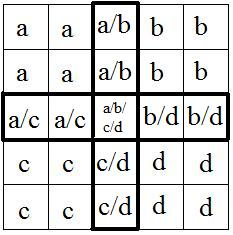
\includegraphics{images/Kuwahara.jpg}
    \caption{The window used by a Kuwahara filter. It is divided into 4 square regions, A, B, C, and D, with the pixels located on the central row and column belonging to more than one region. }
    \label{fig:figure1}
\end{figure}

To find the output of the Kuwahara filter $\Phi$(x,y) for any point (x,y) of the image, we have to calculate the arithmetic mean and the standard deviation of all 4 subregions. Then the new value of the central pixel is given by the arithmetic mean of a subregion where the standard deviation of that subregion must be the smallest of all 4 subregions. 

For color images, the filter should not be performed by applying the filter to each RGB channel separately and recombining the three filtered color channels to form the filtered RGB image. However, the quadrants will have different standard deviations for each channel. Therefore, we have to use the V value from HSV of that image to calculate the standard deviation for each square, so it will let R, G, and B have the same subregion. 

\section{Implementation Progress}
Following the formula, I separated the RGB channel into 3 arrays with the V value I calculated in the RGB to HSV function and recombined the three filtered color channels to form the filtered RGB image. Nevertheless, There are two problems that come up.
\begin{itemize}
  \item Firstly, because the array of each channel is not a contiguous array, I have to convert it to a contiguous array in order to put it into a GPU device.
  \item Secondly, we have to implement the window in (Figure~\ref{fig:figure1}) to a pixel (x,y) in the image. However, the image shape is $(height, width, 3)$, which is have different have a different perspective than the usual x,y coordinate axes (Figure~\ref{fig:figure2}). Because the index in the image is displayed like in Figure~\ref{fig:figure3} so we will have a new perspective when we look at the x,y coordinate axes (Figure~\ref{fig:figure4}).
\end{itemize}. 

\begin{figure}
    \centering
    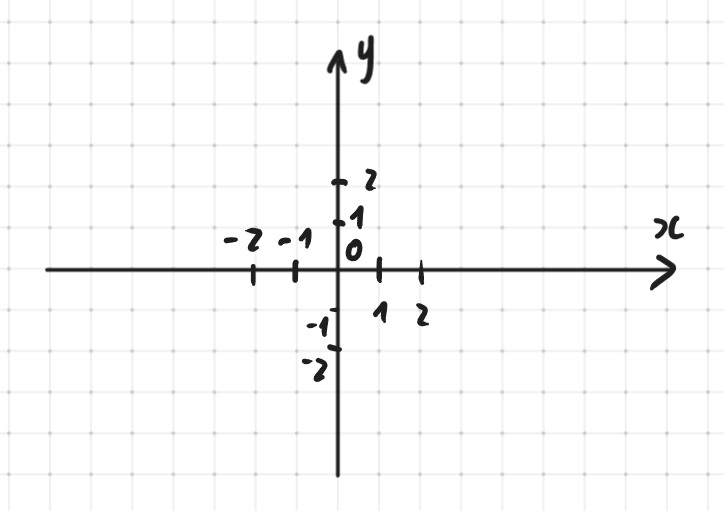
\includegraphics[scale=0.5]{images/normalXY.jpg}
    \caption{Normal x,y coordinate axes}
    \label{fig:figure2}
\end{figure}

\begin{figure}
    \centering
    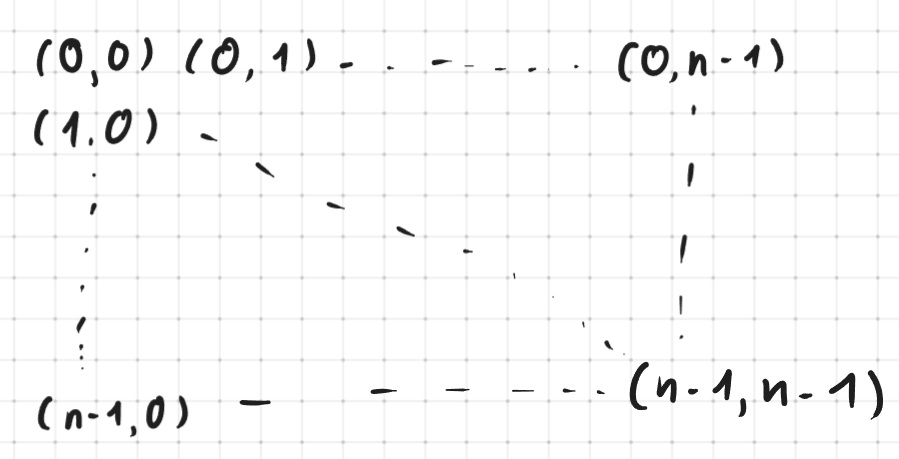
\includegraphics[scale=0.5]{images/imgShape.jpg}
    \caption{Indexs of the image}
    \label{fig:figure3}
\end{figure}

\begin{figure}
    \centering
    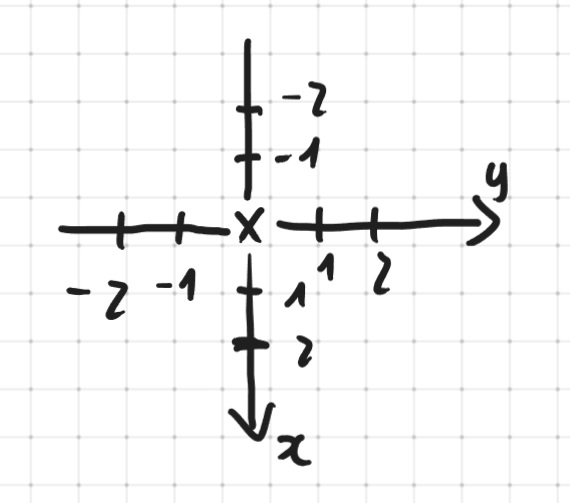
\includegraphics[scale=0.5]{images/newXY.jpg}
    \caption{x,y coordinate axes of the image}
    \label{fig:figure4}
\end{figure}

\pagebreak

Therefore, from the figure above, x is the height, and y is the width of the image when applying it to the function in Cuda Numba. We will have the code for the subregion A of the $\omega$(x,y)

\begin{lstlisting}[language=Python]
winASum = 0
winVASDSum = 0
for i in range(winLen):
    for j in range(winLen):
        xValue = tidx - i
        yValue = tidy - j
        if xValue < 0 or yValue < 0:
            winVASDSum += 0
            winASum += 0
        else:
            winVASDSum += vArr[xValue, yValue]
            winASum += src[xValue, yValue]
\end{lstlisting}

If the value of subregions is out of the border of the image shape (Smaller than 0 or higher than width or height), it will then assign 0 for that position. For example, the code above is subregion A, I am finding the value of each surround pixel value of the central pixel in subregion A of both a V Array and a color channel array. These values will be summed to a variable corresponding to its array winASum, winVASDSum.

\textit{\textbf{Note:} winLen is the length of the small subregion square}

After that, I calculate the arithmetic mean of window V value of A by dividing by the population of window A:

\begin{lstlisting}[language=Python]
meanVA = winVASDSum/((winLen * winLen))
\end{lstlisting}

And so, I calculate the numerator (winVASDSumPow) following the standard deviation formula.

\begin{lstlisting}[language=Python]
winVASDSumPow = 0
for i in range(winLen):
    for j in range(winLen):
        xValue = tidx - i
        yValue = tidy - j
        if xValue < 0 or yValue < 0:
            winVASDSumPow += pow((0 - meanVA),2)
        else:
            winVASDSumPow += pow((vArr[xValue, yValue] - meanVA),2)
\end{lstlisting}

Then use the numerator to calculate the standard deviation:


\begin{lstlisting}[language=Python]
stanA = math.sqrt(winVASDSumPow/((winLen * winLen)))
\end{lstlisting}

These steps repeat three more times, corresponding to 3 other subregions. As a result, we found stanA, stanB, stanC, stanD. And we find min of these four values. 

\begin{lstlisting}[language=Python]
minWin = min(stanA, stanB, stanC, stanD)

if minWin == stanA:
    dst[tidx, tidy] = (winASum/(winLen * winLen))
elif minWin == stanB:
    dst[tidx, tidy] = (winBSum/(winLen * winLen))
elif minWin == stanC:
    dst[tidx, tidy] = (winCSum/(winLen * winLen))
elif minWin == stanD:
    dst[tidx, tidy] = (winDSum/(winLen * winLen))
\end{lstlisting}

The smallest standard deviation value corresponding to which window will lead the arithmetic mean of that window to be the new value of the central pixel.

\section{Result}
In this project, I use winLen = 6 (winLen is the length of a subregion of a window - $\omega$ + 1). 

\begin{lstlisting}[language=Python]
winLen = 6
start = timer()
devBInput = cuda.to_device(np.ascontiguousarray(b))
devBOutput = cuda.device_array((height, width), np.uint8)
kuwa.kuwaFilter_GPU[gridSize, blockSize](devBInput, devBOutput, vArrInput, height, width, winLen)
n_b = devBOutput.copy_to_host()

devGInput = cuda.to_device(np.ascontiguousarray(g))
devGOutput = cuda.device_array((height, width), np.uint8)
kuwa.kuwaFilter_GPU[gridSize, blockSize](devGInput, devGOutput, vArrInput, height, width, winLen)
n_g = devGOutput.copy_to_host()

devRInput = cuda.to_device(np.ascontiguousarray(r))
devROutput = cuda.device_array((height, width), np.uint8)
kuwa.kuwaFilter_GPU[gridSize, blockSize](devRInput, devROutput, vArrInput, height, width, winLen)
n_r = devROutput.copy_to_host()
print("Kuwahara Filter Time: ", timer() - start)

kuwaImgGPU = np.dstack((n_b, n_g, n_r))
\end{lstlisting}

For the result of each channel color, I combined it to become a color RGB image. The figure~\ref{fig:figure5} and figure~\ref{fig:figure6} will show you more about the result.

\begin{figure}
    \centering
    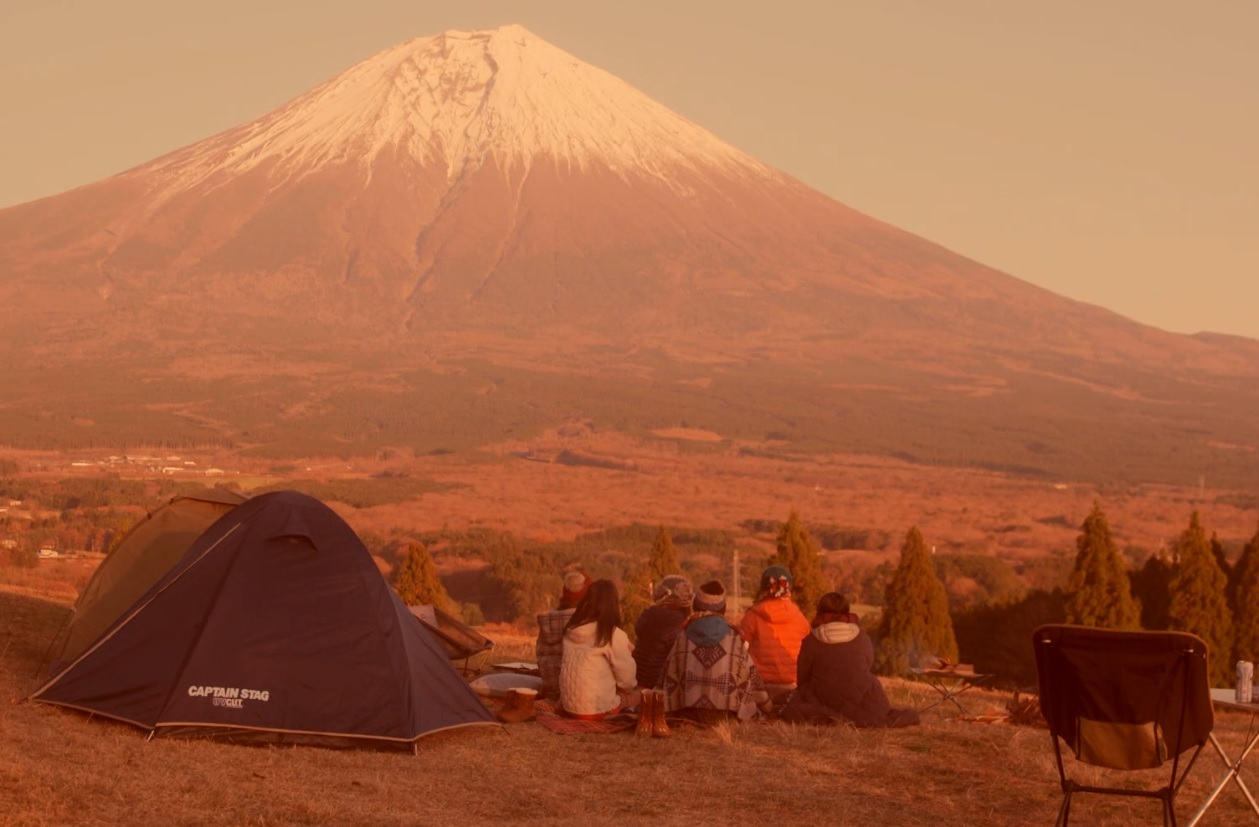
\includegraphics[scale=0.5]{images/yuru.jpg}
    \caption{Original Image}
    \label{fig:figure5}
\end{figure}

\pagebreak

\begin{figure}
    \centering
    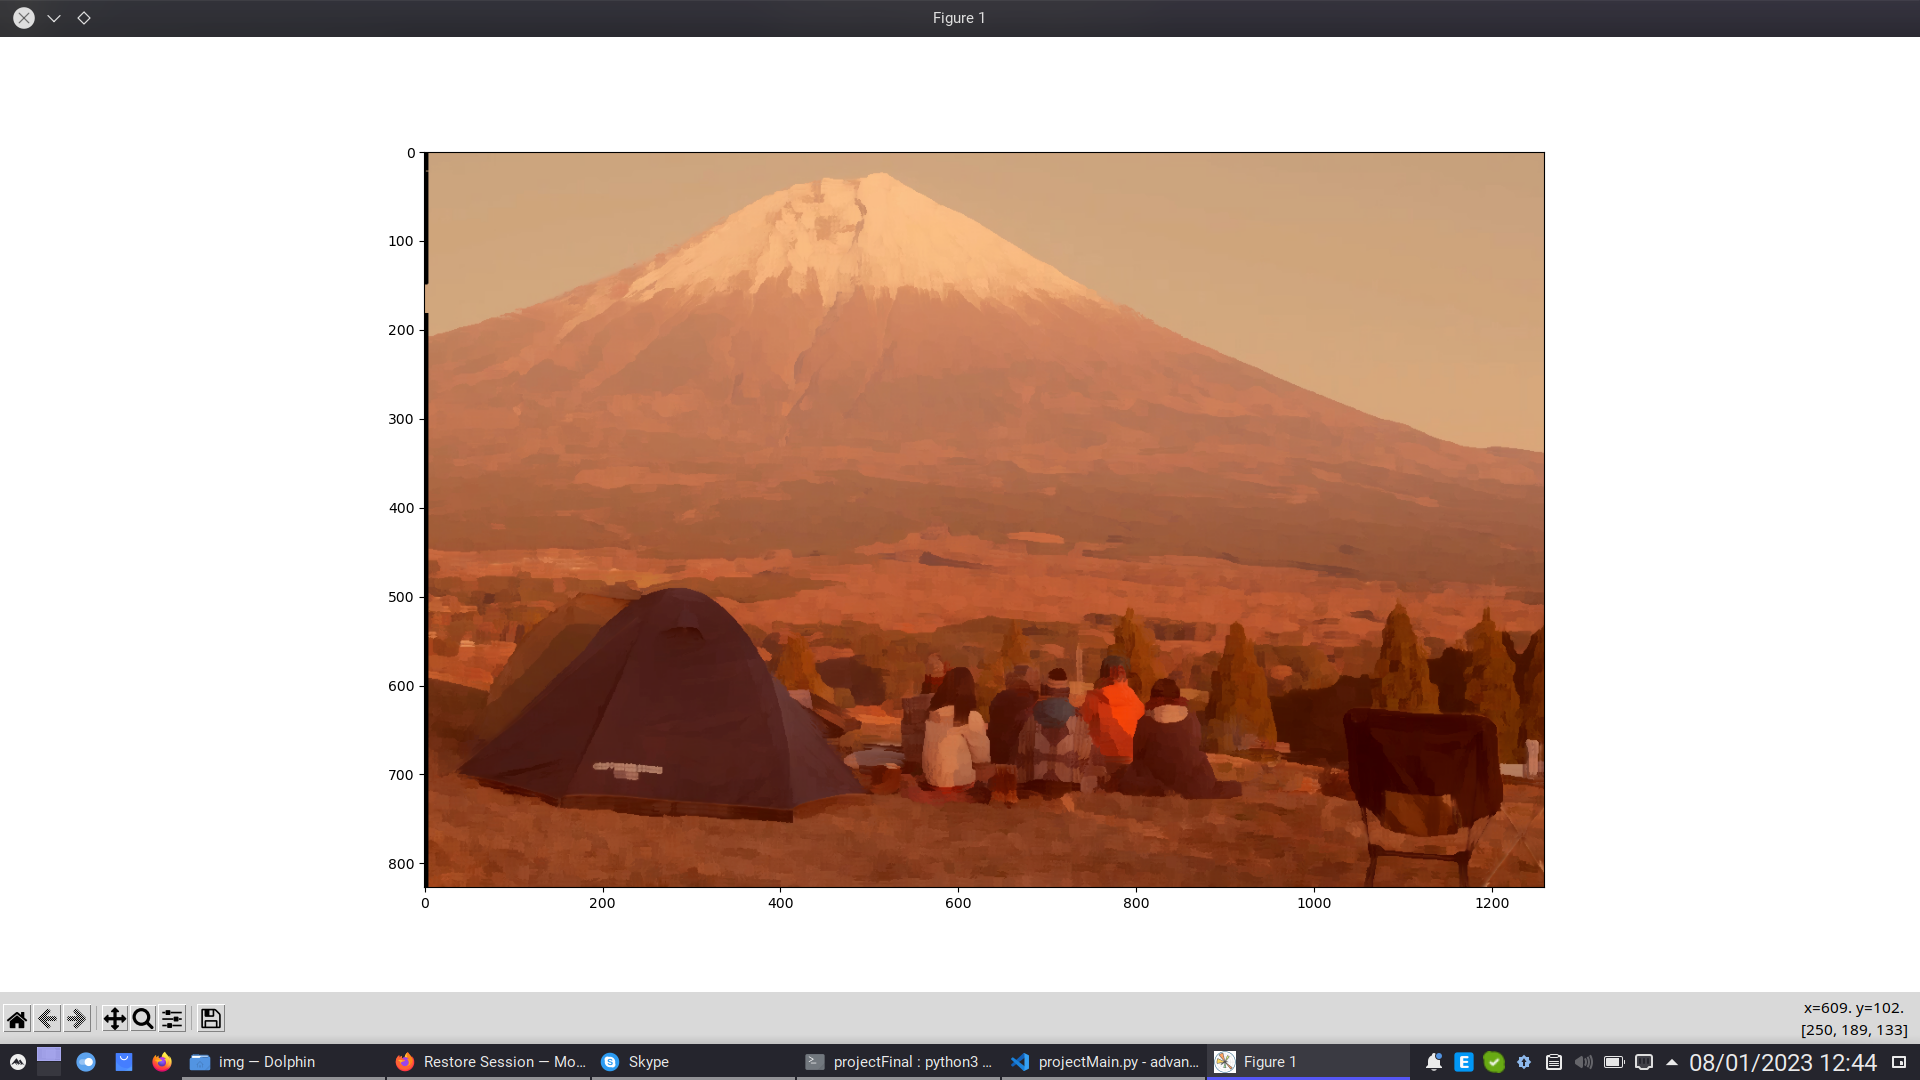
\includegraphics[width= \textwidth]{images/yuruResult.png}
    \caption{After use Kuwahara filter}
    \label{fig:figure6}
\end{figure}

\pagebreak

In the project, I also implement the Kuwahara using CPU. However, it takes a long time to calculate, and for the image 500x500, it takes more than 2 minutes. If using GPU, it will only take 1 second.

Also the project also has a function Kuwahara using GPU but with shared memory. However, the function is not complete and still gives bugs. Currently, if the function does not use cuda.synthread(), it will return a pixelated image. But if I use cuda.synthread(), the project will be run infinitely without stopped. 

\end{document}
